\documentclass[12pt]{article}
\usepackage{graphicx}
\usepackage{float}
\usepackage{amsmath}
\title{Experiment 8: Sequence Generator}
\author{Annirudh K P\\%
210070009}
\date{October 6, 2022}
\begin{document}

\maketitle

\section{Overview of the experiment}
\paragraph{}
In this experiment, we started working on sequential circuit designs using behavourial modelling on VHDL. The problem statement of this experiment is to design a Multiple Strung Detector. The objective of this experiment was to understand the Quartus Design Flow, work with the Xen10 Board, use ScanChain for testbenching, and give us hands on experience over different technical glitches/problems we may face in this piece of software which has been made unwantedly hard.

\section{Experimental Set-up}

\subsection{Design Schematics}
The following state diagram are shown for the Multiple String Detector

\begin{figure}[H]
\centering
  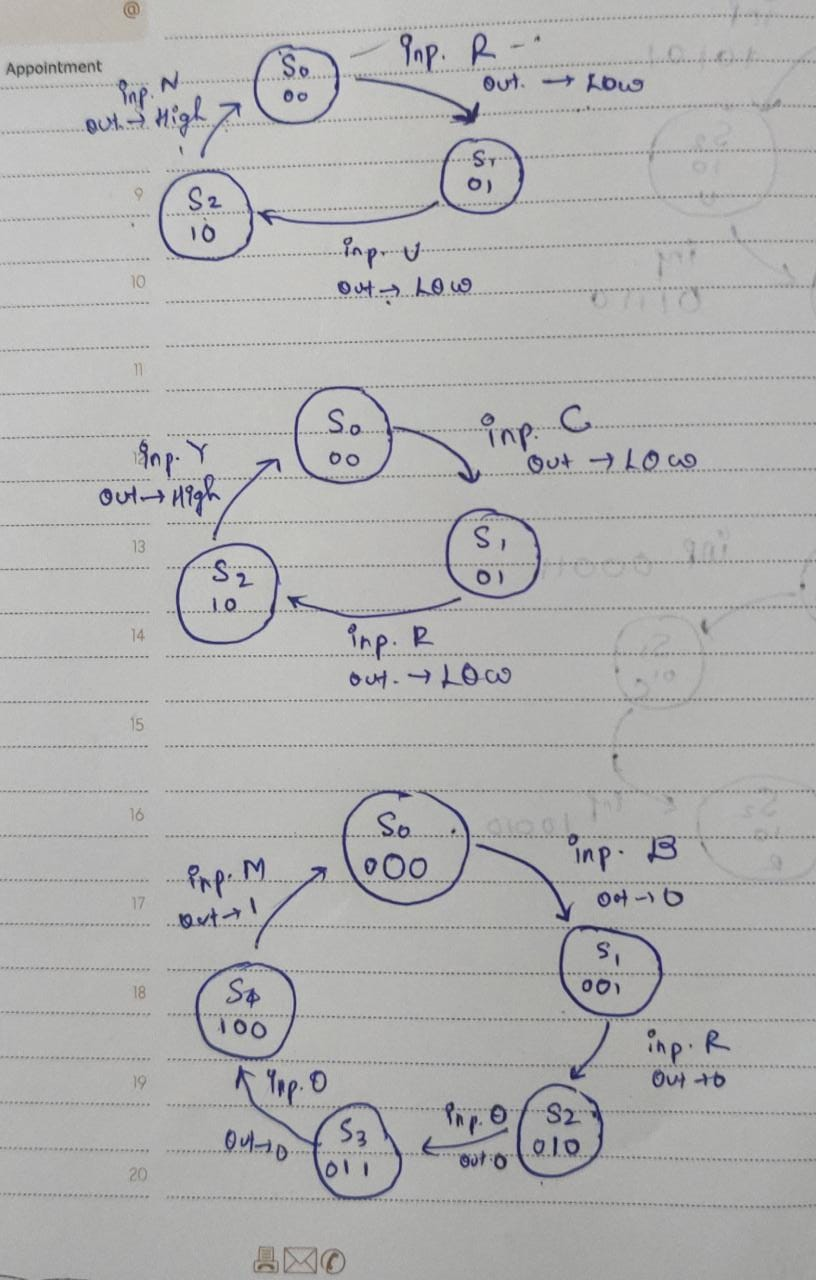
\includegraphics[scale=0.3]{Images/StringDet_Design.jpeg}
  \caption{}
\end{figure}

\subsection{Description of Components}
\subsubsection{Multiple String Generator}
\begin{verbatim}
library ieee;
use ieee.std_logic_1164.all;
use ieee.numeric_std.all;

entity word_detection is
	port( inp:in std_logic_vector(4 downto 0);
		reset,clock:in std_logic;
		outp: out std_logic);
end word_detection;

architecture bhv of word_detection is

---------------Define state type here-----------------------------
type state is (rst1,s11,s12, rst2, s21, s22, rst3, s31, s32, s33, s34); 
---------------Define signals of state type-----------------------
signal y_present1,y_next1: state:=rst1;
signal y_present2,y_next2: state:=rst2;
signal y_present3,y_next3: state:=rst3;
signal outp1, outp2, outp3: std_logic;

begin
clock_proc:process(clock,reset)
begin
	if(clock='1' and clock' event) then
		if(reset = '1') then
			y_present1<= rst1;
			y_present2<= rst2;
			y_present3<= rst3;
		else
			y_present1<= y_next1;
			y_present2<= y_next2;
			y_present3<= y_next3;
		end if;
	end if;
end process;

state_transition_proc:process(inp,y_present1,y_present2,y_present3)
begin
	case y_present1 is
		when rst1=>
			if(unsigned(inp)=18) then --r has been detected
				y_next1<= s11;
			else
				y_next1<=rst1;
			end if;
		when s11=>
			if(unsigned(inp)=21) then --u has been detected
				y_next1<= s12;
			else
				y_next1 <= s11;
			end if;
		when s12=>
			if(unsigned(inp)=14) then --n has been detected
				y_next1<= rst1;
			else
				y_next1<= s12;
			end if;
		when others=>
			null;
	end case;
	
	case y_present2 is
		when rst2=>
			if(unsigned(inp)=3) then --c has been detected
				y_next2<= s21;
			else
				y_next2<=rst2;
			end if;
		when s21=>
			if(unsigned(inp)=18) then --r has been detected
				y_next2<= s22;
			else
				y_next2 <= s21;
			end if;
		when s22=>
			if(unsigned(inp)=25) then --y has been detected
				y_next2<= rst2;
			else
				y_next2<= s22;
			end if;
		when others=>
			null;
	end case;
	
	case y_present3 is
		when rst3=>
			if(unsigned(inp)=2) then --b has been detected
				y_next3<= s31;
			else
				y_next3<=rst3;
			end if;
		when s31=>
			if(unsigned(inp)=18) then --r has been detected
				y_next3<= s32;
			else
				y_next3 <= s31;
			end if;
		when s32=>
			if(unsigned(inp)=15) then --o has been detected
				y_next3<= s33;
			else
				y_next3<= s32;
			end if;
		when s33=>
			if(unsigned(inp)=15) then --o has been detected
				y_next3<= s34;
			else
				y_next3<= s34;
			end if;
		when s34=>
			if(unsigned(inp)=13) then --m has been detected
				y_next3<= rst3;
			else
				y_next3<= s34;
			end if;
		when others=>
			null;
	end case;
end process;

output_proc:process(y_present1, y_present2, y_present3, inp) 
-------the output based on the present state and input (Mealy machine)
begin
	case y_present1 is
		when rst1=>
			outp1<='0';
		when s11=>
			outp1<='0';
		when s12=>
			if (unsigned(inp)=14) then
				outp1<='1';
			else
				outp1<='0';
			end if;
		when others=>
			null;
	end case;
	case y_present2 is
		when rst2=>
			outp2<='0';
		when s21=>
			outp2<='0';
		when s22=>
			if (unsigned(inp)=25) then
				outp2<='1';
			else
				outp2<='0';
			end if;
		when others=>
			null;
	end case;
		case y_present3 is
		when rst3=>
			outp3<='0';
		when s31=>
			outp3<='0';
		when s32=>
			outp3<='0';
		when s33=>
			outp3<='0';
		when s34=>
			if (unsigned(inp)=13) then
				outp3<='1';
			else
				outp3<='0';
			end if;
		when others=>
			null;
	end case;
end process;
outp <= (outp1 or outp2 or outp3);
end bhv;

\end{verbatim}

\section{Observations}
 
We get RTL simulation waveforms for corresponding to input and output which is given below and it shows required results.

\begin{figure}[H]
\centering
  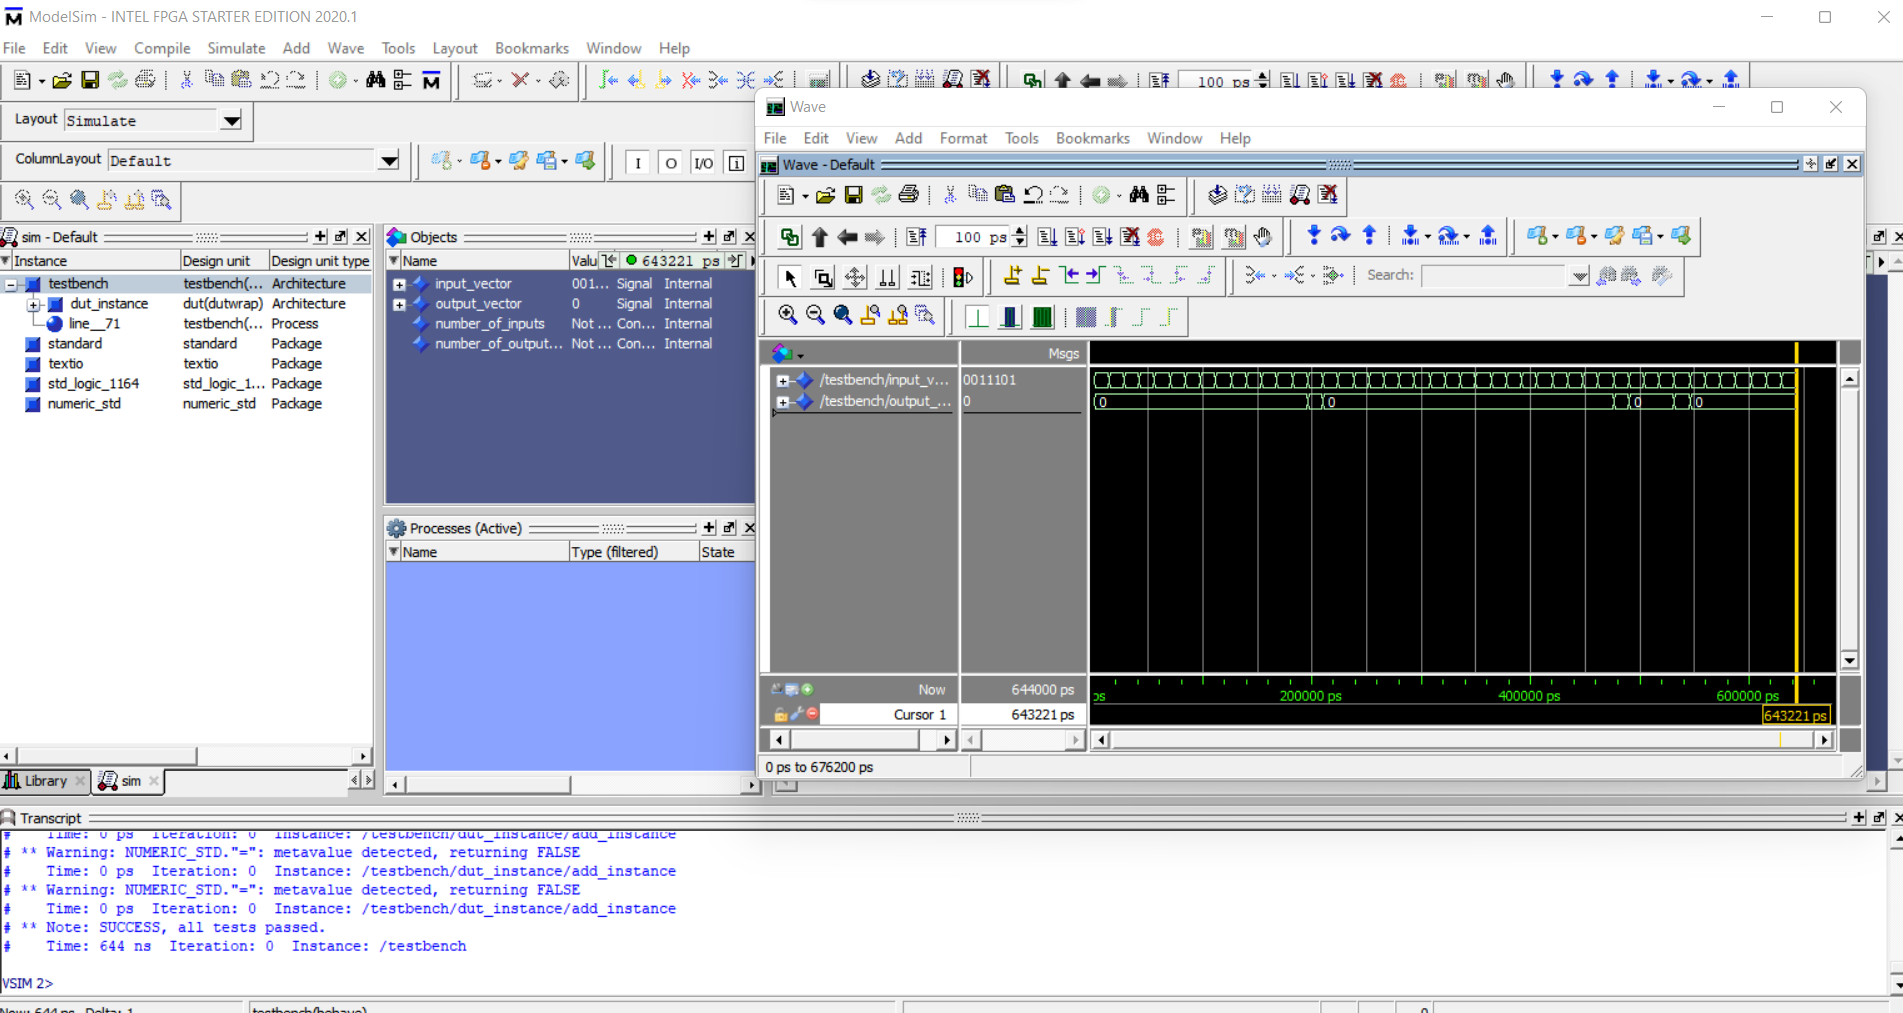
\includegraphics[scale=0.35]{Images/StringDet_RTLSimulation.png}
  \caption{String Detection RTL Simulation Waveform}
\end{figure}

Further the code (in form of .svf file) was flashed onto the Xen10 board. Then scanchain was run to generate outputs using tracefile and then compared to the golden outputs to check if the outputs were indeed correct. The output was verified, which also verified the working of the logic for the Multiple String Detector. The output file's content is shown below.

\begin{verbatim}
0000010 0 Success
0000011 0 Success
0001000 0 Success
0001001 0 Success
1001000 0 Success
1001001 0 Success
0100100 0 Success
0100101 0 Success
0111000 0 Success
0111001 0 Success
0011100 0 Success
0011101 0 Success
1010100 0 Success
1010101 0 Success
0111000 1 Success
0111001 0 Success
0111100 0 Success
0111101 0 Success
0001100 0 Success
0001101 0 Success
0000100 0 Success
0000101 0 Success
1001000 0 Success
1001001 0 Success
0010000 0 Success
0010001 0 Success
1001100 0 Success
1001101 0 Success
0011000 0 Success
0011001 0 Success
1001000 0 Success
1001001 0 Success
0111100 0 Success
0111101 0 Success
0110100 1 Success
0110101 0 Success
0110100 0 Success
0110101 0 Success
1100100 1 Success
1100101 0 Success
0001000 0 Success
0001001 0 Success
0000100 0 Success
0000101 0 Success
0011100 0 Success
0011101 0 Success
\end{verbatim}

\end{document}